\section{\xlabel{nonscience}Processing non-science data\label{se:nonsci}}

This section contains detailed information on how the SCUBA-2 pipeline
processes non-science observations and can be ignored by users only
interested in processing science data. Each of the observation types
are discussed in turn with relevant details on how they are processed
by the different forms of the pipeline.

\subsection{FLATFIELD}

Flatfield data may be taken in a standalone flatfield observation, but
they are also taken as part of science observing, where a fast-ramp
flatfield measurement is made at the beginning and end of the
observation. A flatfield observations consists of a series of
measurements of the bolometer signal in the presence of different
input heater powers, either a set of discrete values or as a series of
continuous ramps alternately increasing and decreasing the heater
power in a sawtooth pattern.

Standalone flatfield observations are processed with the
\task{REDUCE\_FLATFIELD} recipe. A flatfield solution is derived for
each subarray present in each observation and written to an NDF file
with the suffix \verb+_flat+. The pipeline reports the number of good
bolometers and statistics of the responsivities, as well as how they
have changed relative to the existing flatfield solution (i.e.\ that
present in the raw data files). This information is also written to a
log file called \verb+log.flatfield+.

The new solution is also shown and compared with the previous one
graphically. Figure \ref{fig:flatfield} is an example of the
display. The results for each subarray are combined into a focal-plane
mosaic and shown alongside the mosaic for the current
solution. Histograms of the responsivities for the proposed and
current solutions are shown as images side-by-side on the same
scale. In addition a percentage-change image is shown below (scaled
between $\pm10$\,\%), as well as histograms of the new and existing
responsivities (again on the same scale).

\begin{figure}[t]
\centering
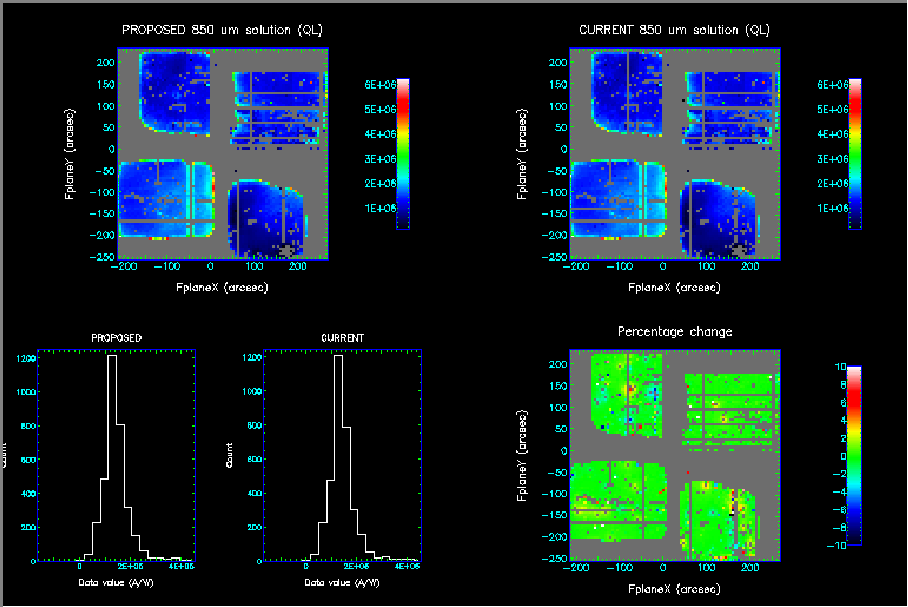
\includegraphics[width=\textwidth]{sun264_flatfield}
\caption{Example display from a FLATFIELD observation or FASTFLAT
  sequence. The top left panel is the responsivity map for this
  observation (containing the proposed new solution), the top right
  panel shows the current responsivity solution (i.e\ currently in
  use) for comparison. The bottom left panels are responsivity
  histograms for this observation and the current solution (PROPOSED
  and CURRENT respectively). The bottom right panel shows the
  percentage change in the responsivities between this observation and
  the current solution in use, scaled between
  $\pm10$\,\%.\label{fig:flatfield}}
\end{figure}

Once complete, the pipeline writes a flag file in
\verb+ORAC_DATA_OUT+ for the current observation containing the name
of each successful flatfield solution. The flag file is a hidden file
with the name \verb+.sYYYYMMDD_MMMMM.ok+ where \verb+YYYYMMDD+ is the
UT date and \verb+MMMMM+ is the zero-padded observation number. This
file is used by the telescope control system (TCS) at the JCMT to
identify the new flatfields to use in subsequent observations.

\subsubsection{Fast-ramps}

The fast-ramp flatfields (FASTFLAT) taken as part of on-sky observing
are included with the science data and processed as part of
map-making, but may be processed separately using the
\task{REDUCE\_FASTFLAT} recipe to assess how much the responsivities
change during an observation. The results are calculated and displayed
as above, but in this case the second fast-ramp flatfield is compared
with the first, and not with the internal flatfield solution.

Fast-ramp flatfields are also processed separately in the QL and
summit pipelines and picked up as necessary for map-making or noise
calculations.

\subsection{NOISE}

Noise observations are a series of measurements recording the
bolometer signal either against a dark shutter or open to the
atmosphere. The telescope is not tracking a source during the
measurement. The recipe calculates the average power spectrum of each
array. The \SMURF\ task \task{calcnoise} is used to calculate the
noise properties for each subarray between 2 and 10\,Hz. The recipe
calibrates the noise data using the appropriate FCF to calculate the
noise equivalent flux density (NEFD). If the measurement is on sky,
the NEFD is also quoted for the zenith, using the current optical
depth and airmass.

A numerical summary of the noise properties, showing the mean, median
and modal noise values, the effective noise equivalent power and
number of bolometers, is written to the screen. These results are also
written to a log file called \verb+log.bolonoise+. The NEFD results
are written to a log file called \verb+log.nefd+.

Focal-plane mosaics of the noise, the percentage change in the noise
since the last measurement and the NEP are displayed in a Kapview
window along with a histogram of the noise values (see
Fig.~\ref{fig:noise}).

The QL and summit pipelines process each file as it is written to
disk. Otherwise all of the data (for a given subarray) are passed to
\task{calcnoise}.

\begin{figure}[t]
\centering
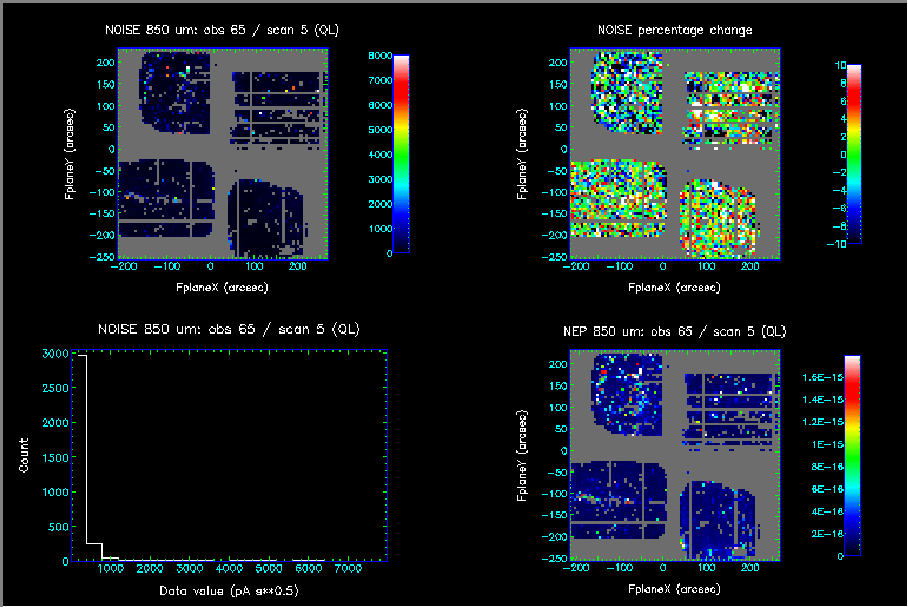
\includegraphics[width=\textwidth]{sun264_noise}
\caption{Example display from a NOISE observation. The top-left panel
  displays the noise for the current data, while the top-right panel
  shows the percentage change since the previous noise
  measurement. The bottom-left panel shows a histogram of noise
  values, while the bottom-right shows the NEP for the current
  data.\label{fig:noise}}
\end{figure}

\subsection{POINTING}

Pointing observations consist of making a map of a point source, and
are processed with the \task{REDUCE\_POINTING} recipe. The recipe
processes the data with the iterative map-maker, crops the image to
75\,arcsec on a side and removes any residual large-scale background
signal with \CUPID\ \task{findback}. If the source is a known
calibrator, the pipeline derives an FCF.

The name of the processed image is written into a flag file (as for
FLATFIELD observations above). The flag file is read by the telescope
POINTING\_FOCUS task which analyzes the named image to calculate the
pointing offsets applied to the telescope pointing model.

The pipeline makes its own estimate of the pointing offsets in two
ways by applying a point-source filter (matched filter) to enhance the
signal-to-noise ratio in the image followed by fitting a 2-D profile
to the source and calculating the centroid position. Both results are
written to a log file called \verb+log.pointing+.

The pipeline displays the image used to derive the pointing offsets in
a \GAIA\ window. The recipe also fits a 2-d profile to the source and
writes the result to a log file called \verb+log.beam+.

The map-maker uses the config file \verb+dimmconfig_pointing.lis+,
except for very short pointing observations (defined as $<15$\,s)
which use \verb+dimmconfig_veryshort_planet.lis+ for planets and
\verb+dimmconfig_bright_compact_veryshort.lis+ for all other sources.

The QL pipeline uses the \task{REDUCE\_POINTING\_QL} recipe, which
contains different logic for dealing with DREAM and STARE data but is
functionally identical to the main \task{REDUCE\_POINTING} recipe for
SCAN data.

\subsection{FOCUS}

Focus observations are processed with the \task{REDUCE\_FOCUS}
recipe. A focus observation consists of a series of maps made of a
point source with the secondary mirror (SMU) at various
positions. Only one axis (either X, Y or Z) is varied at a time.

In the QL pipeline, the maps are made as the data are taken and
collated once the observation has ended. (In practice, due to the fact
that the QL pipeline cannot rely on the \verb+OBSEND+ FITS header, an
observation is considered to have ended once an image exists at each
of the SMU positions: the number of SMU positions is retrieved from
the FITS header.) The non-QL pipeline processes each SMU setting in
turn.

Once all the maps exist, the pipeline creates a cube with the third
axis given by the SMU position. The images are registered to the same
pixel coordinates before adding to the cube so that they align
correctly.

The pipeline writes a flag file (as above) which contains the name of
the data cube. The flag file is read by the telescope POINTING\_FOCUS
task which analyzes the cube to calculate the best SMU position. The
pipeline makes its own estimate of the best-fit SMU position by
fitting a parabola to the peak fluxes derived from 2-D fits (provided
at least three fluxes could be derived) and writes that number to a
log file called \verb+log.focus+.

The images at each focus position are displayed in sequence in a
single Kapview window (see Figure \ref{fig:focus}).

\begin{figure}[t]
\centering
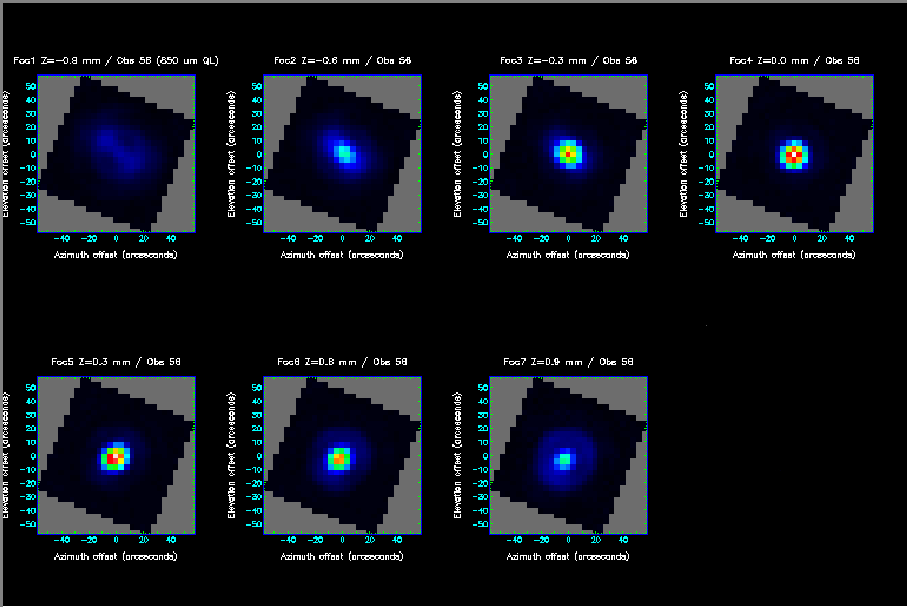
\includegraphics[width=\textwidth]{sun264_focus}
\caption{Example display from a FOCUS observation showing a reduced
  image for each of seven SMU positions. The SMU position (and axis)
  is given in the title for each image. The images are displayed with
  axes of arcsecond offsets.\label{fig:focus}}
\end{figure}

The map-maker uses either the \verb+dimmconfig_veryshort_planet.lis+
for planets and \\ \verb+dimmconfig_bright_compact_veryshort.lis+ for
all other sources.

The same recipe is used for all forms of the pipeline. The output cube
has the suffix \verb+_foc+.

\subsection{SETUP}

A SETUP observation consists of a fast-ramp flatfield (FASTFLAT)
measurement followed by a NOISE, both taken with the shutter
closed. The recipe processes each separately as described for the
respective observation types above. The results of processing each
type of data are displayed in separate Kapview windows. The pipeline
writes a flag file at the end of the observation with the names of the
files containing the names of the flatfield solutions and noise
calculations for the telescope software to read.

\subsection{SKYDIP}

A SKYDIP observation is a series of NOISE-SKY observations at
differing airmass. Currently there is no pipeline recipe to process
these data, other than as a NOISE observation.
